\documentclass{article}
\usepackage[margin=0.6in]{geometry}
\usepackage{amsmath}
\usepackage{amssymb}
\usepackage{bookmark}
\usepackage{graphicx}
\usepackage{float}

\newcommand{\vct}[1]{\mathbf{#1}}
\newcommand{\argmax}{\mathop{\mathrm{argmax}}}
\newcommand{\argmin}{\mathop{\mathrm{argmin}}}

\title{Solutions to the Assignment - 5 : CS5560 - \\
Probabilistic Models in Machine Learning}
\author{Vishwak Srinivasan\\
\texttt{CS15BTECH11043}}
\date{}

\begin{document}
\maketitle

\section*{Implementation of Bayes Classifier and Naive-Bayes Classifier}
\begin{flushleft}
The accuracies of the Bayes Classifier and the Naive-Bayes Classifier on the dataset were the same and were equal to \(93.4211\%\). Surprisingly, this was also the accuracy of the trained logistic regression classifier using \texttt{LIBLINEAR}. The misclassified examples by the Bayes classifier and Naive-Bayes classifier are reported below:
\begin{center}
\begin{tabular}{|p{0.2\linewidth}|p{0.6\linewidth}|}
\hline
Bayes & 36, 160, 161, 176, 203, 219, 239, 251, 254, 257, 259, 263, 267, 274, 275, 278, 280, 282, 284, 285, 286, 296, 297, 300, 302, 304, 305, 306, 309, 316, 319, 323, 324, 328, 330, 335, 337, 340, 341, 342, 344, 349, 351, 352, 354, 357, 364, 377, 379, 381, 384, 386, 390, 392, 398, 401, 404, 405, 407, 411, 414, 419, 421, 422, 423, 425, 428, 431, 434, 438, 439, 443, 445, 446, 448, 453, 465, 472, 473, 494, 503, 505, 518, 533, 535, 554, 555, 557, 566, 570, 590, 594, 597, 608, 613, 614, 618, 629, 633, 640, 650, 653, 655, 692, 693, 695, 696, 697, 701, 710, 713, 716, 718, 720, 722, 733, 802, 909, 1111, 1193, 1207, 1373, 1386, 1487, 1495, 1500, 1522, 1549, 1553, 1569, 1612, 1635, 1669, 1673, 1687, 1691, 1701, 1703, 1724, 1732, 1738, 1740, 1762, 1786, 1826, 1836, 1839, 1953, 1963, 1985, 2002, 2046, 2152, 2155, 2209, 2210, 2230, 2250, 2261, 2285, 2292, 2298, 2311, 2340, 2402, 2448, 2513, 2523, 2543, 2554\\
\hline
Naive-Bayes & 36, 160, 161, 176, 203, 219, 239, 251, 254, 257, 259, 263, 267, 274, 275, 278, 280, 282, 284, 285, 286, 296, 297, 300, 302, 304, 305, 306, 309, 316, 319, 323, 324, 328, 330, 335, 337, 340, 341, 342, 344, 349, 351, 352, 354, 357, 364, 377, 379, 381, 384, 386, 390, 392, 398, 401, 404, 405, 407, 411, 414, 419, 421, 422, 423, 425, 428, 431, 434, 438, 439, 443, 445, 446, 448, 453, 465, 472, 473, 494, 503, 505, 518, 533, 535, 554, 555, 557, 566, 570, 590, 594, 597, 608, 613, 614, 618, 629, 633, 640, 650, 653, 655, 692, 693, 695, 696, 697, 701, 710, 713, 716, 718, 720, 722, 733, 802, 909, 1111, 1193, 1207, 1373, 1386, 1487, 1495, 1500, 1522, 1549, 1553, 1569, 1612, 1635, 1669, 1673, 1687, 1691, 1701, 1703, 1724, 1732, 1738, 1740, 1762, 1786, 1826, 1836, 1839, 1953, 1963, 1985, 2002, 2046, 2152, 2155, 2209, 2210, 2230, 2250, 2261, 2285, 2292, 2298, 2311, 2340, 2402, 2448, 2513, 2523, 2543, 2554\\
\hline
\end{tabular}
\end{center}
\end{flushleft}

\section*{Exercises from ML: A Probabilistic Perspective}
\subsection*{Exercise 4.19}
\begin{flushleft}
There are no assumptions considered on the parameters \(\pi_{0}, \pi_{1}\), \(\mu_{0}, \mu_{1}\) and \(\Sigma_{0}, \Sigma_{1}\) except for the fact that \(\Sigma_{1} = k\Sigma_{0}\) and \(\pi_{0} = 1 - \pi_{1}\).

Note that:
\begin{gather}
(\vct{x} - \mu_{1})^{T}\Sigma_{1}^{-1}(\vct{x} - \mu_{1}) = \frac{1}{k}(\vct{x} - \mu_{1})^{T}\Sigma_{0}^{-1}(\vct{x} - \mu_{1})\\
|2\pi \Sigma_{1}|^{-0.5} = k^{-\frac{n}{2}} |2\pi \Sigma_{0}|
\end{gather}

This means that:
\begin{multline}
p(y = 1 | \vct{x}; \theta) = \frac{\pi_{1}|2\pi \Sigma_{1}|^{-0.5} \exp(\frac{-1}{2}\left((\vct{x} - \mu_{1})^{T}\Sigma_{1}^{-1}(\vct{x} - \mu_{1})\right)}{\pi_{1}|2\pi \Sigma_{1}|^{-0.5} \exp(\frac{-1}{2}\left((\vct{x} - \mu_{1})^{T}\Sigma_{1}^{-1}(\vct{x} - \mu_{1})\right) + \pi_{0}|2\pi \Sigma_{0}|^{-0.5} \exp(\frac{-1}{2}\left((\vct{x} - \mu_{0})^{T}\Sigma_{0}^{-1}(\vct{x} - \mu_{0})\right)}\\= \frac{\pi_{1}k^{-\frac{n}{2}} \left(\exp(\frac{-1}{2}\left((\vct{x} - \mu_{1})^{T}\Sigma_{0}^{-1}(\vct{x} - \mu_{1})\right)\right)^{\frac{1}{k}}}{\pi_{1}k^{-\frac{n}{2}} \left(\exp(\frac{-1}{2}\left((\vct{x} - \mu_{1})^{T}\Sigma_{0}^{-1}(\vct{x} - \mu_{1})\right)\right)^{\frac{1}{k}} + (1 - \pi_{1}) \exp(\frac{-1}{2}\left((\vct{x} - \mu_{0})^{T}\Sigma_{0}^{-1}(\vct{x} - \mu_{0})\right)}
\end{multline}

A special case arises if \(\mu_{1} = \mu_{0}\):
\begin{equation}
p(y = 1 | \vct{x} ; \theta) = \frac{\pi_{1} k^{-\frac{n}{2}}}{\pi_{1} k^{-\frac{n}{2}} + (1 - \pi_{1}) (f^{\frac{k - 1}{k}}_{\mu_{0}, \Sigma_{0}}(\vct{x}))}
\end{equation}
where \(f_{\mu_{0}, \Sigma_{0}}(\vct{x}) = \exp(\frac{-1}{2}(\vct{x} - \mu_{0})^{T}\Sigma_{0}^{-1}(\vct{x} - \mu_{0}))\)
\end{flushleft}

\subsection*{Exercise 4.21}
\subsubsection*{Part a}
\begin{flushleft}
If \(p(x | \mu_{1}, \sigma_{1}) \geq p(x | \mu_{2}, \sigma_{2})\), then \(-2\log p(x | \mu_{1}, \sigma_{1}) \leq -2\log p(x | \mu_{2}, \sigma_{2})\). This means that:
\begin{equation}
\label{r1-eqn}
\frac{(x - \mu_{1})^{2}}{\sigma_{1}^{2}} + \log \sigma_{1}^{2} \leq \frac{(x - \mu_{2})^{2}}{\sigma_{2}^{2}} + \log \sigma_{2}^{2} \Rightarrow x^2 - \frac{(x - 1)^{2}}{10^{6}} - \log (10^{6}) \leq 0 \Rightarrow x^{2}\left(1 - \frac{1}{10^{6}}\right) + x\frac{2}{10^{6}} - \left(\frac{1}{10^{6}} + \log 10^{6}\right) \leq 0
\end{equation}

A graphical sketch is shown below:
\(\newline\)
\begin{minipage}{0.475\linewidth}
\begin{figure}[H]
\centering
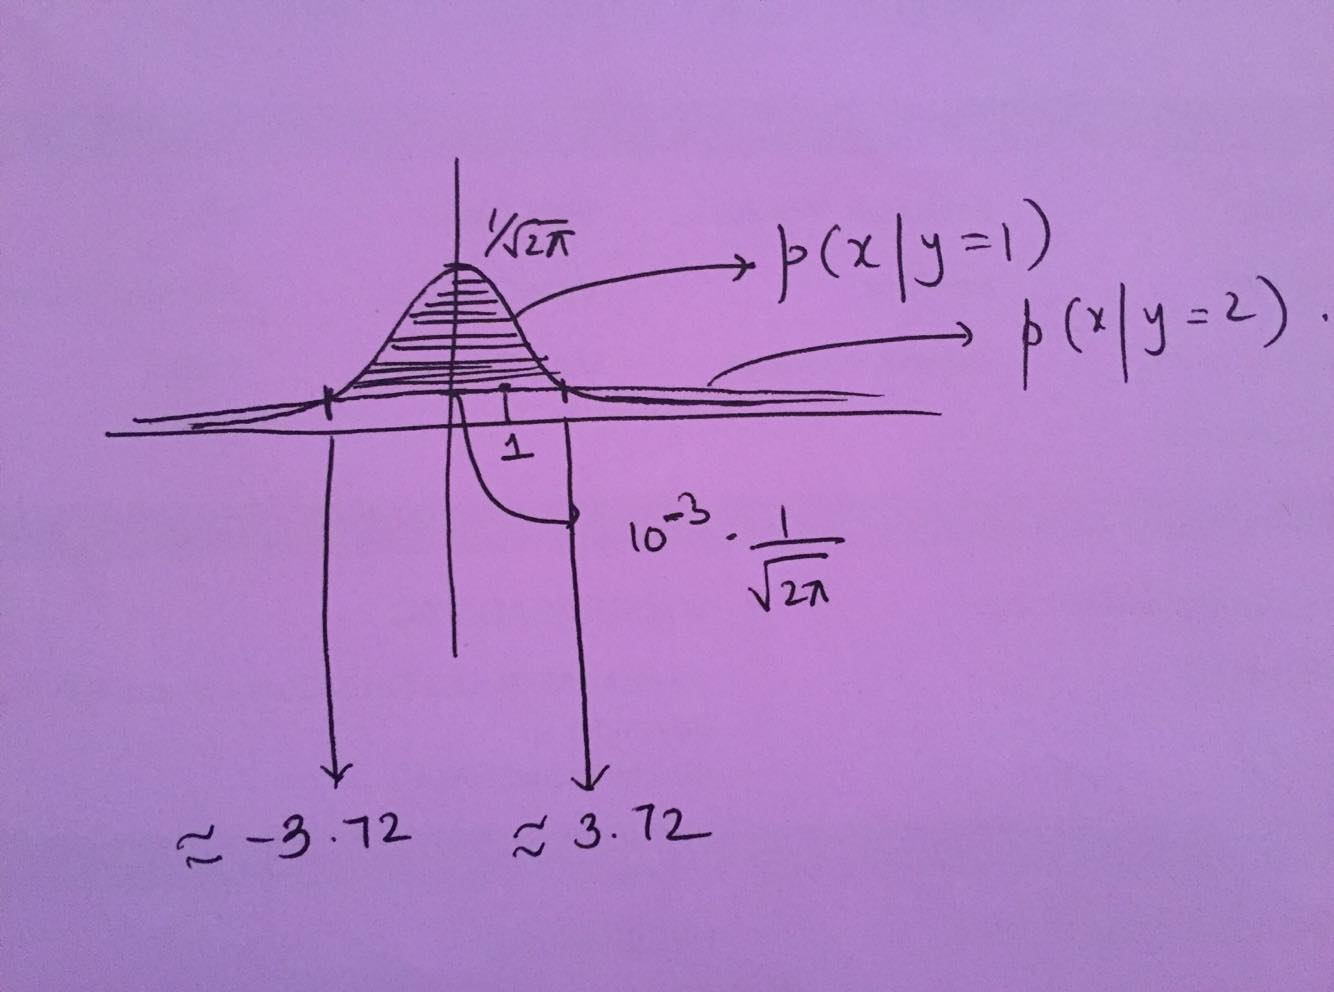
\includegraphics[width=0.6\textwidth]{./images/4_21_a_sketch.jpg}
\end{figure}
\end{minipage}
\hfill
\begin{minipage}{0.475\linewidth}
The domain of the shaded region corresponds to the set \(R_{1}\). The end-points of this domain can be found by solving the equality case in \ref{r1-eqn}. Denote \(C_{1} = 1 - \frac{1}{10^{6}}\), \(C_{2} = \frac{2}{10^{6}}\) and \(C_{3} = -\left(\frac{1}{10^{6}} + \log 10^{6}\right)\).
\begin{multline}
C_{1}x^2 + C_{2}x + C_{3} = 0 \Rightarrow x = \frac{-C_2 \pm \sqrt{C_{2}^{2} - 4C_{1}C_{3}}}{2C_{1}}\\= \frac{-1 \pm 10^{3}\sqrt{10^{6}\log 10^{6} + 1 - \log 10^{6}}}{(10^{6} - 1)}\\\Rightarrow x \approx \pm 3.7169
\end{multline}
\end{minipage}
\end{flushleft}

\subsubsection*{Part b}
\begin{flushleft}
Note that if \(\sigma_{1}^{2} = \sigma_{2}^{2}\), then the first equality in \ref{r1-eqn} would become:
\begin{equation}
(x - \mu_{1})^{2} \leq (x - \mu_{2})^{2} \Rightarrow 2(\mu_{2} - \mu_{1})x \leq \mu_{2}^{2} - \mu_{1}^{2} \Rightarrow x \leq \frac{\mu_{2} + \mu_{1}}{2} = \frac{1}{2}
\end{equation}

\begin{minipage}{0.475\linewidth}
\begin{figure}[H]
\centering
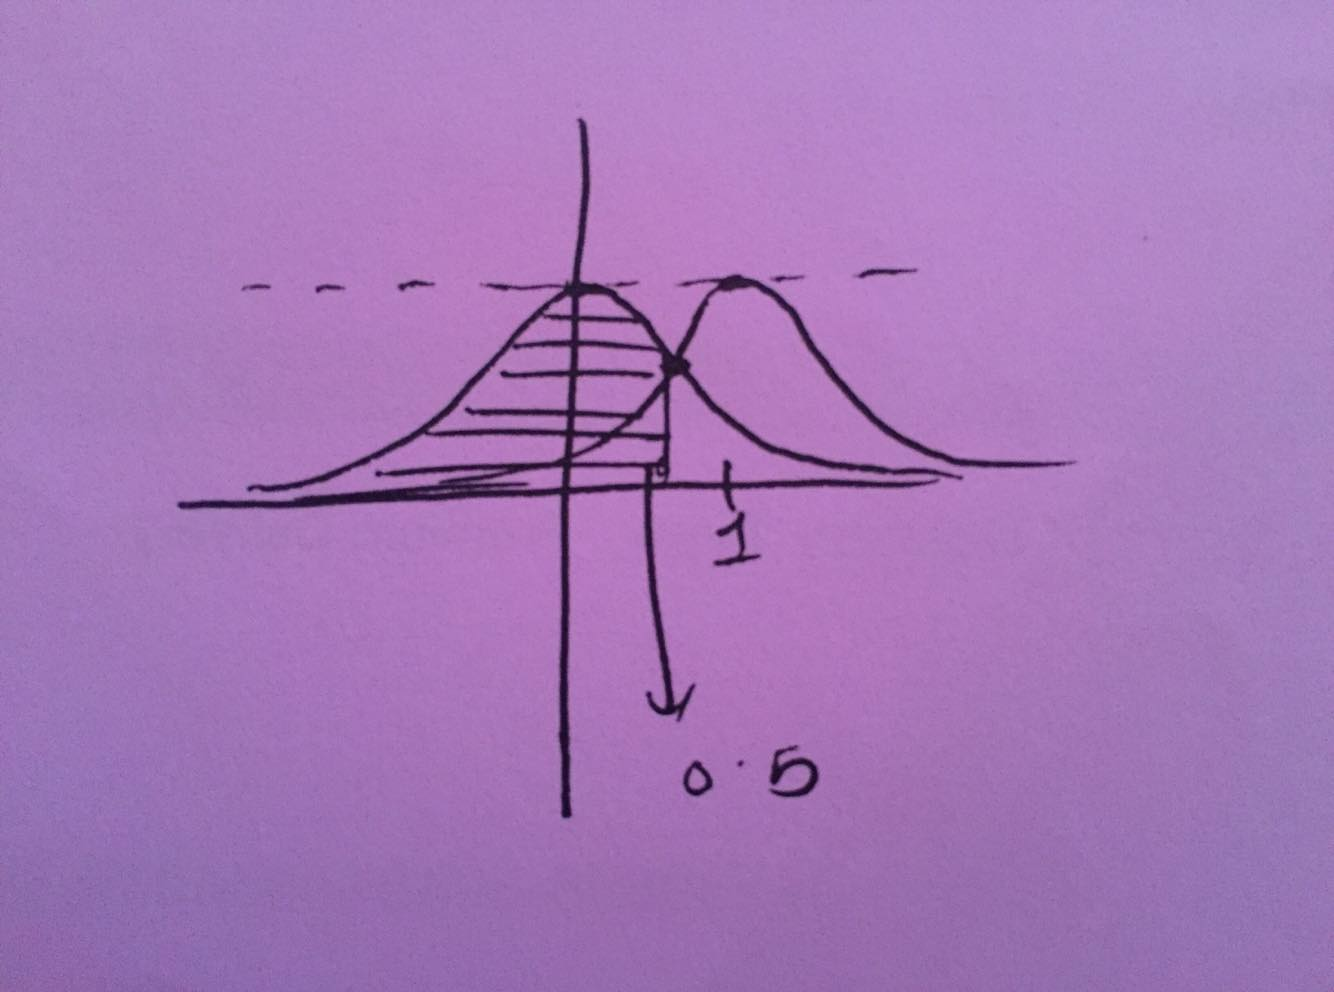
\includegraphics[width=0.6\textwidth]{./images/4_21_b_sketch.jpg}
\end{figure}
\end{minipage}
\hfill
\begin{minipage}{0.475\linewidth}
\(R_{1}\) is the left partition of the real line from \(\frac{1}{2}\).
\end{minipage}
\end{flushleft}

\subsection*{Exercise 4.22}
\begin{flushleft}
Recall that the predictor is given by \(\hat{g}(\vct{x}) = \argmax_{y \in \mathcal{Y}} p(Y | \vct{x} = y)\). Now from the facts in the question:
\begin{equation}
p(y | \vct{x}) \propto p(\vct{x} | y) p(y) \propto p(\vct{x} | y)
\end{equation}

The last proportionality excludes \(p(y)\) due to the fact that the \(P(Y = 1) = P(Y = 2) = P(Y = 3) = \frac{1}{3}\). Now the prediction equation can be re-written as:
\begin{equation}
\hat{g}(\vct{x}) = \argmax_{y \in \{1, 2, 3\}} p(\vct{x} | Y = y) = \argmax_{y \in \{1, 2, 3\}} \log p(\vct{x} | Y = y) = \argmin_{y \in \{1, 2, 3\}} -2\log p(\vct{x} | Y = y) - 2\log 2\pi
\end{equation}

Some equations to consider:
\begin{gather}
-2\log p(\vct{x} | Y = i) - 2\log 2\pi= (\vct{x} -\vct{\mu}_{1})^{T}\Sigma^{-1}_{1}(\vct{x} -\vct{\mu}_{1}) + \log |\Sigma_{i}|
\end{gather}

\begin{center}
\begin{tabular}{|c|c|c|}
\hline
\(i\) & \(\Sigma_{i}^{-1}\) & \(|\Sigma_{i}|\) \\
\hline
\(1\) & \(\begin{bmatrix} \frac{1}{0.7} & 0 \\ 0 & \frac{1}{0.7} \end{bmatrix}\) & \(0.49\) \\
\hline
\(2\) & \(\begin{bmatrix} \frac{4}{3} & -\frac{1}{3} \\ -\frac{1}{3} & \frac{4}{3} \end{bmatrix}\) & \(0.6\) \\
\hline
\(3\) & \(\begin{bmatrix} \frac{4}{3} & -\frac{1}{3} \\ -\frac{1}{3} & \frac{4}{3} \end{bmatrix}\) & \(0.6\) \\
\hline
\end{tabular}
\end{center}

\subsubsection*{Part a}
\begin{equation}
\hat{g}([-0.5, 0.5]) = \argmin_{y \in \{1, 2, 3\}} \{0.0009, 2.3225, 0.3225\} = 1
\end{equation}

\subsubsection*{Part b}
\begin{equation}
\hat{g}([0.5, 0.5]) = \argmin_{y \in \{1, 2, 3\}} \{0.0009, -0.0108, 3.3225\} = 2
\end{equation}
\end{flushleft}

\section*{Starred Problems}
\subsection*{Problem 1: 4.20 from ML: A Probabilistic Perspective}
Please note that the loss function \(L(M)\) in the question is an optimization problem over the log-posterior probabilities. Therefore, discriminative models will have achieved the best possible fit (global optimum) due to the formulation being a concave problem (convex after simplification). This means that \texttt{LinLog} and \texttt{QuadLog} will be the best models (comparison between these made later in part c).
\subsubsection*{Part a}
\begin{flushleft}
Note that \texttt{GaussI} is a generative model. Hence from the above argument, \(L(\texttt{GaussI}) \leq L(\texttt{LinLog})\).
\end{flushleft}

\subsubsection*{Part b}
\begin{flushleft}
Note that \texttt{GaussX} is a generative model. Hence from the above argument, \(L(\texttt{GaussX}) \leq L(\texttt{QuadLog})\).
\end{flushleft}

\subsubsection*{Part c}
\begin{flushleft}
Now, it is easy to see that \texttt{LinLog} is a special case of \texttt{QuadLog}, where the quadratic coefficients are 0. This means that \texttt{QuadLog} has more expressivity than \texttt{LinLog}, hence \(L(\texttt{LinLog}) \leq L(\texttt{QuadLog})\).
\end{flushleft}

\subsubsection*{Part d}
\begin{flushleft}
From the same argument in Part a and b, we can say that \(L(\texttt{GaussI}) \leq L(\texttt{QuadLog})\).
\end{flushleft}

\subsubsection*{Part e}
\begin{flushleft}
This statement is true if the datapoints are separable. The reason is because of the fact that maximizing \(L(M)\) would bring about boundary that separates these classes to be as far away from the boundary as possible. This means that the classification error is also effectively reduced due to the existence of such a boundary.
\end{flushleft}

\subsection*{Problem 2: 8.6 from ML: A Probabilistic Perspective}
\subsubsection*{Part a}
\begin{flushleft}
First we prove that \(f(\vct{w}) = -\log \sigma(y \vct{x}^{T} \vct{w})\) is convex. Now:
\begin{gather}
\frac{df}{dw_{i}} = -\frac{1}{\sigma(y \vct{x}^{T}\vct{w})} \sigma(y \vct{x}^{T}\vct{w}) (1 - \sigma(y \vct{x}^{T}\vct{w})) yx_{i} = (\sigma(y \vct{x}^{T}\vct{w}) - 1) yx_{i}\\
\frac{d^{2}f}{dw_{i}dw_{j}} = yx_{i}\sigma(y \vct{x}^{T}\vct{w})(1 - \sigma(y \vct{x}^{T}\vct{w}))yx_{j}
\end{gather}

Consider \(\vct{z}\) such that \(\vct{z} \neq 0\). Now we know that the matrix formed with the \((ij)^{th}\) entry as \(\frac{d^{2}f}{dw_{i}dw_{j}}\) is the Hessian (denoted by \(\vct{H}\)). To prove that this function is convex, we have to show that \(\vct{z}^{T}\vct{H}\vct{z} \geq 0\) or \(\displaystyle\sum_{i, j = 1} z_{i}z_{j}H_{ij} \geq 0\). We will use the second approach.
\begin{multline}
\sum_{i}\sum_{j} z_{i}z_{j}y^{2}x_{i}x_{j}\sigma(y \vct{x}^{T}\vct{w})(1 - \sigma(y \vct{x}^{T}\vct{w})) = y^{2}\sigma(y \vct{x}^{T}\vct{w})(1 - \sigma(y \vct{x}^{T}\vct{w}))\left(\sum_{i}z_{i}x_{i}\right)\left(\sum_{j}z_{j}x_{j}\right)\\= \sigma(y \vct{x}^{T}\vct{w})(1 - \sigma(y \vct{x}^{T}\vct{w})) \left(\sum_{i} z_{i}x_{i}\right)^{2} > 0
\end{multline}

The final step is due to:
\begin{enumerate}
\item \(y^{2} = 1\) for \(y = \{+1, -1\}\)
\item \(\sigma(y \vct{x}^{T}\vct{w}) \in (0, 1) \Rightarrow 1 - \sigma(y \vct{x}^{T}\vct{w}) \in (0, 1) \Rightarrow \sigma(y \vct{x}^{T}\vct{w})(1 - \sigma(y \vct{x}^{T}\vct{w})) > 0\)
\item \(\displaystyle\sum_{i}\sum_{j} a_{i}a_{j} = \sum_{i}a_{i}\sum_{j}a_{j} = \left(\sum_{i}a_{i}\right)\left(\sum_{i}a_{i}\right) = \left(\sum_{i}a_{i}\right)^{2} > 0\) for non-zero \(\vct{a}\).
\end{enumerate}

Next the sum of two strictly convex functions are convex. Define \(h(x) = f(x) + g(x)\) where \(f\) and \(g\) are strictly convex. Using Jensen's inequality, for \(\lambda \in [0, 1]\):
\begin{multline}
h(\lambda x_{1} + (1 - \lambda)x_{2}) = f(\lambda x_{1} + (1 - \lambda)x_{2}) + g(\lambda x_{1} + (1 - \lambda)x_{2})\\< \lambda f(x_{1}) + (1 - \lambda)f(x_{2}) + g(x_{1}) + (1 - \lambda)g(x_{2})\\= \lambda(f(x_{1}) + g(x_{1})) + (1 - \lambda)(f(x_{2}) + g(x_{2}))=\lambda h(x_{1}) + (1 - \lambda)h(x_{2})
\end{multline}

This can be generalized for as many functions as we want via induction, which means that \(\displaystyle\sum_{i \in \mathcal{D}} -\log \sigma(y_{i}\vct{x}_{i}^{T}\vct{w})\) is strictly convex as well. Scaling by a positive constant doesn't affect strict convexity, hence \(\displaystyle\frac{1}{|\mathcal{D}|}\sum_{i \in \mathcal{D}} -\log \sigma(y_{i}\vct{x}_{i}^{T}\vct{w})\) is strictly convex as well. Trivially, for \(\lambda > 0\), \(\lambda ||\vct{w}||_{2}^{2}\) is convex, meaning that \(J(\vct{w})\) is strictly convex. Therefore, \(J(\vct{w})\) cannot have multiple optimal solutions. The statement is \textbf{false}.
\end{flushleft}

\subsubsection*{Part b}
L2 regularization can be perceived as optimizing over a circle (in 2D). The critical points attained at the boundary are not sparse, unlike L1 regularization which can be perceived as optimizing over a diamond figure (in 2D), where the points of at which low norm is achieved are the corners of the diamond, effectively nullifying some of the dimensions. The statement is \textbf{false}

\subsubsection*{Part c}
\textbf{True}, as explained in class.

\subsubsection*{Part d}
Increasing the \(\lambda\) parameter, will cause the weights to approach \(0\) more, since the problem is biased towards giving solutions with low norm. This could cause the other component of \(J(\vct{w})\) which is \(-\ell(\vct{w}, \mathcal{D}_{\text{train}})\) to increase. This would hence cause \(\ell(\vct{w}, \mathcal{D}_{\text{train}})\) to decrease. The statement is \textbf{false}.

\subsubsection*{Part e}
Increasing the \(\lambda\) parameter, will cause low-norm (biased) solutions. However, it is not exactly clear if this will be good for the testing set, even though it is clear it is not good for the training set, and hence may not always be the case. The statement is \textbf{false}.

\subsection*{Problem 3: 8.7 from ML: A Probabilistic Perspective}
\subsubsection*{Part a}
\begin{minipage}{0.475\linewidth}
\begin{figure}[H]
\centering
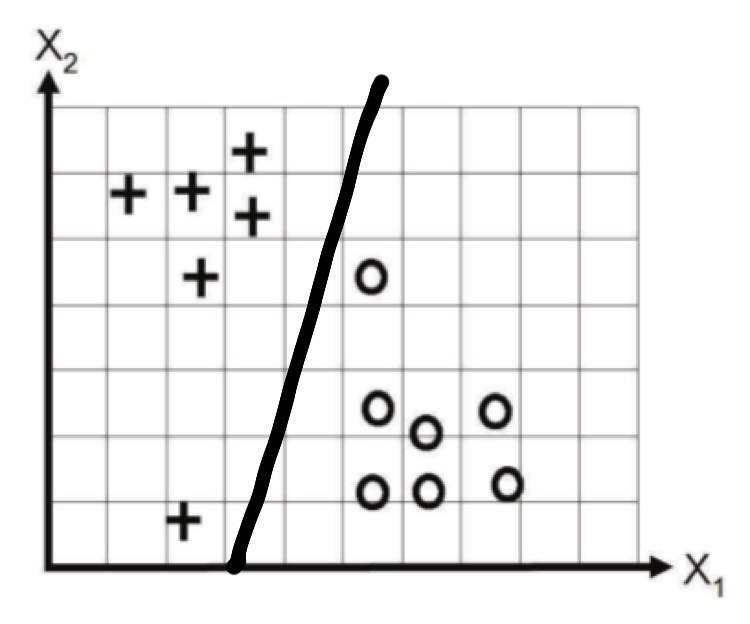
\includegraphics[width=0.6\textwidth]{./images/8_7_a.jpg}
\end{figure}
\end{minipage}
\hfill
\begin{minipage}{0.475\linewidth}
The boundary is basically the line \(w_{0} + w_{1}x_{1} + w_{2}x_{2} = 0\). Now, scaling the weights will not affect this boundary, meaning that the drawn line is not the unique solution for the problem. There are no classification errors made on the training dataset.
\end{minipage}

\subsubsection*{Part b}
\begin{minipage}{0.475\linewidth}
\begin{figure}[H]
\centering
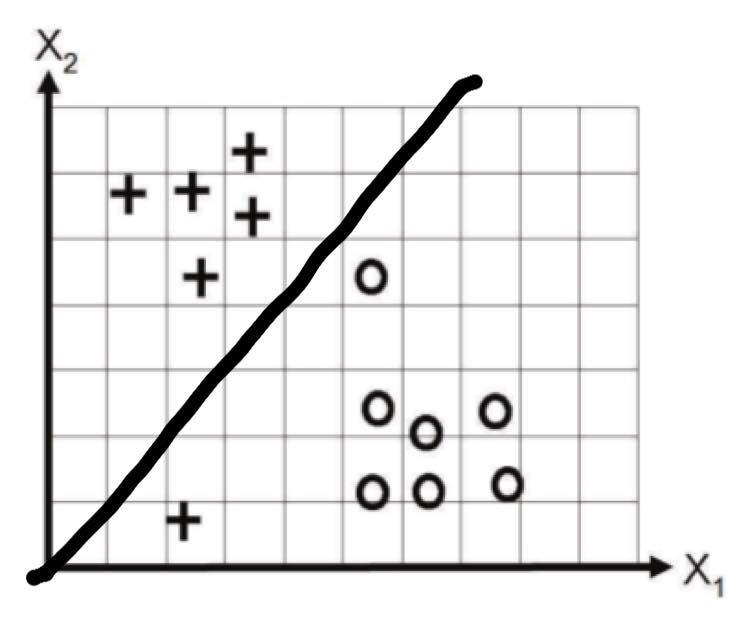
\includegraphics[width=0.6\textwidth]{./images/8_7_b.jpg}
\end{figure}
\end{minipage}
\hfill
\begin{minipage}{0.475\linewidth}
The boundary is basically the line \(w_{0} + w_{1}x_{1} + w_{2}x_{2} = 0\). Since the intercept term is regularized down to 0, the boundary would be a line very close / passing through the origin. There will be one classification error.
\end{minipage}

\subsubsection*{Part c}
\begin{minipage}{0.475\linewidth}
\begin{figure}[H]
\centering
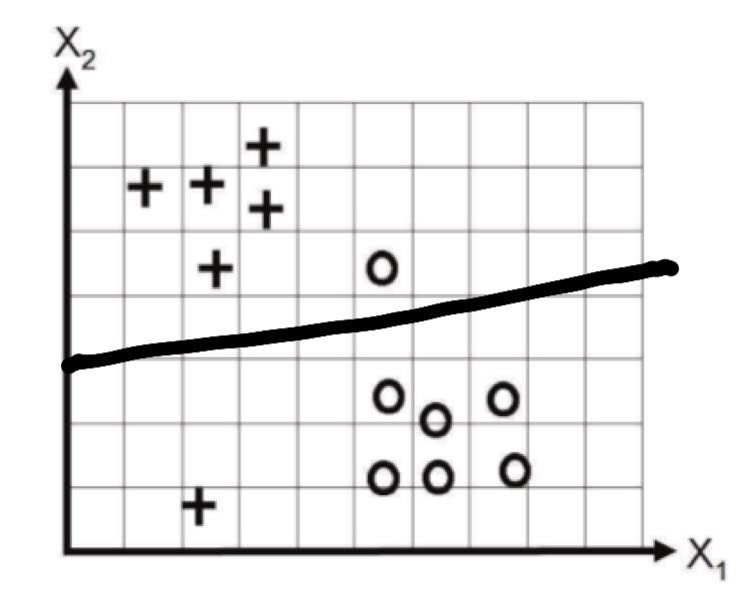
\includegraphics[width=0.6\textwidth]{./images/8_7_c.jpg}
\end{figure}
\end{minipage}
\hfill
\begin{minipage}{0.475\linewidth}
The slope of the line \(w_{0} + w_{1}x_{1} + w_{2}x_{2} = 0\) is \(-\frac{w_{1}}{w_{2}}\). Since there is control over the parameter \(w_{1}\), the slope will also be controlled, and possibly close to \(0\) too. There will be two classification errors.
\end{minipage}

\subsubsection*{Part d}
\begin{minipage}{0.475\linewidth}
\begin{figure}[H]
\centering
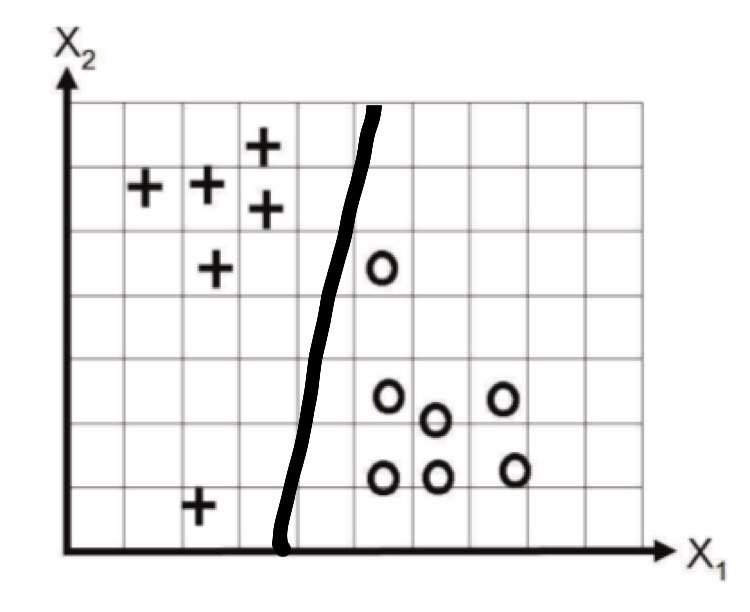
\includegraphics[width=0.6\textwidth]{./images/8_7_d.jpg}
\end{figure}
\end{minipage}
\hfill
\begin{minipage}{0.475\linewidth}
The slope of the line \(w_{0} + w_{1}x_{1} + w_{2}x_{2} = 0\) is \(-\frac{w_{1}}{w_{2}}\). Since there is control over the parameter \(w_{2}\), the slope could possibly be very high in magnitude, thus causing a boundary to be more ``parallel'' to the vertical axis. There will be no classification errors.
\end{minipage}
\end{document}
